%%%%%%%%%%%%%%%%%%%%%%%%%%%%%%%%%%%%%%%%%%%%%%%%%%%%%%%%%%%%%%%%%%%%%
% Section: Computational Footprinting with HMMs
%%%%%%%%%%%%%%%%%%%%%%%%%%%%%%%%%%%%%%%%%%%%%%%%%%%%%%%%%%%%%%%%%%%%%
\subsection{Computational Footprinting with HMMs}
\label{sec:computational.footprinting.hmms}

% TODO
% In this section we will describe how we applied the HMMs to the problem of detection of active TFBSs

% Figure - footprinting with HMMs
\begin{figure}[h!]
\centering
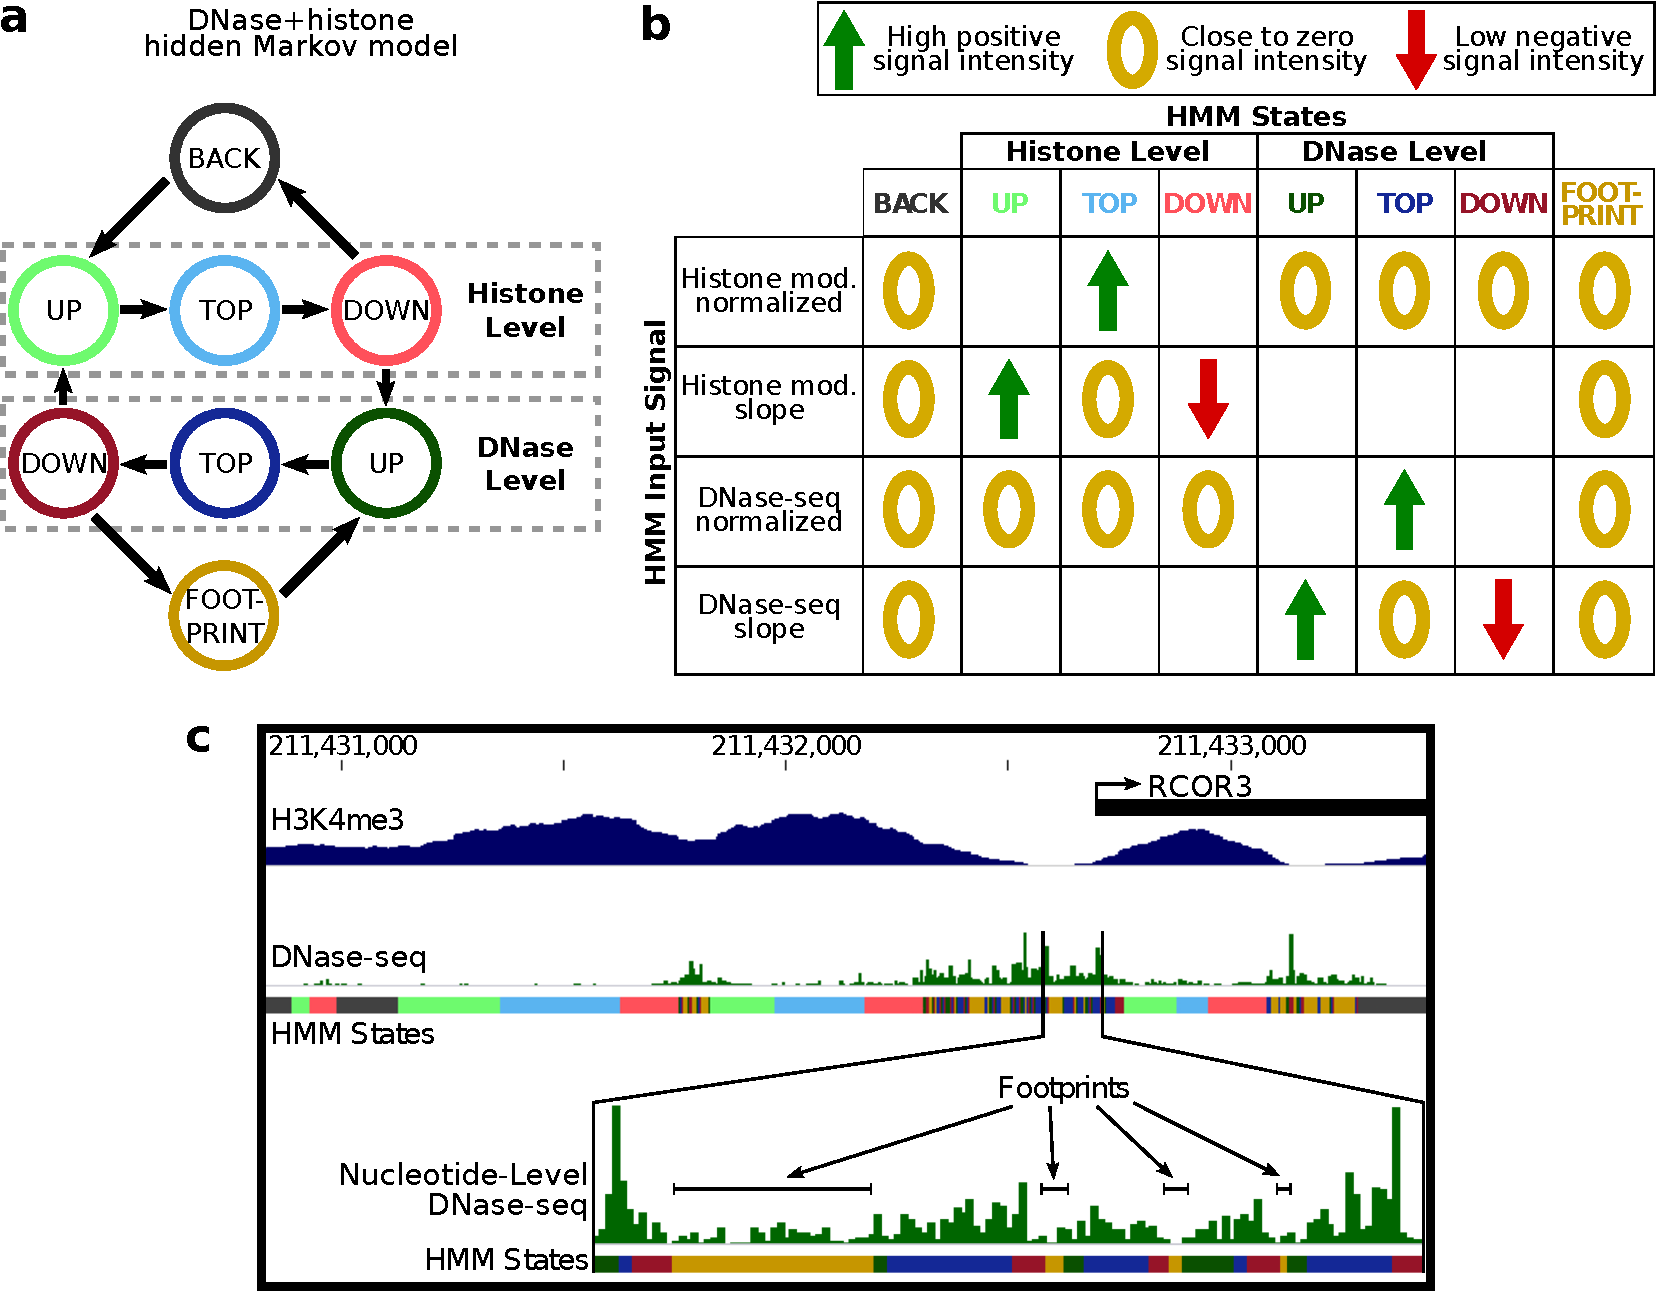
\includegraphics[width=0.99\textwidth]{gusmao_hmm_footprinting}
\caption[Computational footprinting with HMMs]{\textbf{Computational footprinting with HMMs.} (\textbf{a}) DNase-seq and H3K4me3 (ChIP-seq) profiles around the promoter region of RCOR3 -- REST corepressor 3 on K562 cell type. The DNase-seq signal indicates three clear regions of DHS (HS1, HS2 and HS3), each of which fits dip regions within the H3K4me3 signal. Moreover, these regions consist of several putative footprints of varied sizes. (\textbf{b}) Eight state HMM proposed. The first state models background signal ({\tt BACK}). From the background state, the only possible transition is to the histone level states, which will model the increase ({\tt UP}), high levels ({\tt TOP}) and decrease ({\tt DOWN}) of histone modifications. After visiting histone level states, the HMM allows transitions to the DNase level states, which again model the increase, high levels and decrease in the DHS signal. Only then, the {\tt FOOTPRINT} state can be visited. After a footprint visit, the HMM has to go again to the DNase and histone level states, emphasizing the peak-dip-peak pattern. We omit the self-transitions, which are present in all states, for simplicity.}
\label{fig:gusmao_hmm_footprinting}
\end{figure}

%%%%%%%%%%%%%%%%%%%%%%%%%%%%%%%%%%%%%%%%%%%%%%%%%%%%%%%%%%%%%%%%%%%%%
% Section: HMM Topology and Parameters
%%%%%%%%%%%%%%%%%%%%%%%%%%%%%%%%%%%%%%%%%%%%%%%%%%%%%%%%%%%%%%%%%%%%%
\subsubsection{HMM Topology and Parameters}
\label{sec:hmm.yopology.parameters}

% TODO

The HMM structure was designed to recognize the epigenetic grammar
described in Section~\ref{sec:our.approach}. This segmentation task is
performed based on four input signals: the normalized and slope versions
of both DHS and a histone modification. The structure,
depicted in Figure~\ref{fig:gusmao_hmm_footprinting}b can be interpreted as follows.
The first state ({\tt BACK}) corresponds to the `background' regions
with low concentration of DHS and histone marks. The
histone level states represent a peak in the histone modification signal,
recognizing an increase in the histone modification signal based on high positive
slope values ({\tt UP}), summit regions with slope
values close to zero with high normalized values ({\tt TOP}) and a
decrease based on negative values of the slope signal ({\tt DOWN}).
From the histone level {\tt DOWN} state, the model can either return
to {\tt BACK} (isolated histone modification peaks without further DHS) or continue
to the DNase level {\tt UP} state. The DNase
level states are equivalent to the histone level states, with the
exception that the DHS normalized and slope signals are being
recognized instead. From the DNase level {\tt DOWN} state, the model
decides between returning to a region of higher histone
modification signals (histone level {\tt UP} state) and visiting the
{\tt FOOTPRINT} state, which represents the dip between two peaks of
intense DHS. The regions of the genome where the HMM has
recognized as {\tt FOOTPRINT} are the ones reported by our method as
likely TFBSs. See Supplementary Section~3.3 for alternative HMM topologies.

More formally, for an observed multivariate sequence $\mathbf{X}$ and
a hidden variable $\mathbf{Q}=\{q_1,...,q_N\}$, we can describe an HMM
by parameters $\Theta= A,B,\Pi\}$. $A$ represents the state
transition matrix
\begin{equation}
    A = {\{a_{uv}\}}^{S \times S},
\end{equation}
where~$S$ is the number of states and $a_{uv}$ represents the
probability of transition from state $u$ to $v$. The initial state
transition probabilities are represented as
\begin{equation}
    \Pi = \{\pi_{1},...,\pi_{S}\}.
\end{equation}
We use a multivariate normal density function with full covariance matrix as emission probability
of the states. For a given genomic position $j$ and state $u$ we have
\begin{equation}
    \begin{array}{lcl}
p(\mathbf{x_{\cdot j}}|q_j=u) & = & p(\mathbf{x_{\cdot j}}|{{\mu}^{u}},{{\Sigma}^{u}})\\[0.4em]
                          & = &
\frac{1}{ \sqrt{(2\pi)^{D} {| {{{\Sigma}^{u}}} |}}}
e^{-\frac{1}{2} (\mathbf{x_{\cdot j}}-\mu^u)^T (\Sigma^u)^{-1} (\mathbf{x_{\cdot j}}-\mu^u)}, \\
    \end{array}
    \label{eq:gaussian}
\end{equation}
where $\mu^u$ and $\Sigma^u$ are respectively the $D$-dimensional
mean vector and full covariance matrix. Lastly, the emission parameters $B$ are
defined as $\{(\mu^1,\Sigma^1),...,(\mu^S,\Sigma^S)\}$.

%%%%%%%%%%%%%%%%%%%%%%%%%%%%%%%%%%%%%%%%%%%%%%%%%%%%%%%%%%%%%%%%%%%%%
% Section: HMM Training and Decoding
%%%%%%%%%%%%%%%%%%%%%%%%%%%%%%%%%%%%%%%%%%%%%%%%%%%%%%%%%%%%%%%%%%%%%
\subsubsection{HMM Training and Decoding}
\label{sec:hmm.training.decoding}

% Theory

The HMM is trained with maximum likelihood parameters on a supervised
approach. For a given annotation sequence of the hidden data $\mathbf{Q}$ and
sample data $\mathbf{X}$, the parameters are estimated as
\begin{equation}
    a_{uv} = \frac{ \alpha^{\prime}_{uv}}{ \sum_{w=1}^{S} \alpha^{\prime}_{uw}},
    \label{eq:train1}
\end{equation}
where $\alpha^{\prime}_{uv}=\sum_i^{N-1} \mathbf{1} (q_i=u,q_{i+1}=v)$
represents the number of transitions from state~$u$ to state~$v$
observed in the training data. 

As we expect the HMM to always start at the {\tt BACK} state, the initial
transition vector $\pi_1=1$ and $\pi_u=0$ for $u > 1$. 

Finally, the emission parameters are estimated as
\begin{equation}
\mu^{u} = \frac{ \sum_{j=1}^{N} {x}_{\cdot j} {\mathbf{1}}(q_j=u) }{ \sum_{j=1}^{N} {\mathbf{1}} (q_j=u) },
    \label{eq:train2}
\end{equation}
and
\begin{equation}
    {\Sigma}^{u} =  \frac{ \sum_{j=1}^{N} ({x}_{\cdot j} - {\mu}^{u})^T({x}_{\cdot j} - {\mu}^{u}) {\mathbf{1}} (q_j=u)}
                         { \sum_{j=1}^{N} {\mathbf{1}} (q_j=u)  - 1}.
    \label{eq:train3}
\end{equation}

The final goal of our model is to find the most probable states
visited for a given genomic signal. More formally, we want to find the
most probable sequence of hidden states $ \mathbf{Q}$ having
observed~$\mathbf{X}$ given a model~$ \Theta$, which can be written as
\begin{equation}
    \mathbf{Q^*} = \argmax{\mathbf{Q}} p\left(\mathbf{X},\mathbf{Q}|\Theta\right).
    \label{eq:viterbi1}
\end{equation}
The solution to the above problem is given by the Viterbi algorithm~\cite{rabiner1989}.
In practical terms, we consider positions annotated with the {\tt FOOTPRINT}
state to be potential active TFBSs.

% In practise

To reduce the dimensionality of the data, we first applied a peak calling tool
to find regions with evidence of DHS and histone modification signals. The enriched
regions of histone modifications ChIP-seq data were defined using the peak-calling
tool MACS~\cite{zhang2008}. We used a $p$-value of $ 10^{-5} $ and all default
parameters from MACS 1.4. No further filtering, such as false discovery rate, was
performed on the peaks, as we wanted a lenient selection of candidate regions. The
enriched regions of the DHS data were defined as in~\cite{boyle2011}. Briefly, a
signal corresponding to the estimated density of the DHS is generated by applying F-seq
software~\cite{boyle2008b} to the DNase-seq mapped reads and background information
based on alignability, copy number and karyotype correction. A threshold is then
calculated by fitting the signal to a gamma distribution and considering the value
that corresponds to a loose $p$-value of $ 0.01 $. We merge all enriched regions
for a given cell type and extend them by 5000 bp in each direction. This step keeps
only $3-6\%$ of the genome with DHS or histone modification evidence for a given
cell type (see Supplementary Table~5 for complete statistics).

We selected a 10,000 bp region around the promoter of the gene RCOR3 and performed
a cell type-specific manual annotation with one of the 8 HMM states according to the
epigenetic grammar described in Figure~\ref{fig:gusmao_hmm_footprinting}. As one of the histones marks
-- H3K4me1 -- is known to be associated to distal enhancers, we have additionally
annotated an enhancer region. The selection of these regions was made randomly, but
we checked ENCODE tracks for evidence that the gene RCOR3 was expressed in all cell types
analyzed and that the enhancer region was far ($>$100kb) from known genes and expressed
regions.

In order to help the annotation of the footprints, MPBSs with all PWMs from Jaspar,
Transfac and Uniprobe datasets were detected inside the training regions. We consider
(active) footprints all the signal depleted regions between two DHS peaks that overlap
a MPBS. We trained five HMMs per cell type, one for each histone modification (H3K4me3, H3K9ac,
H3K29ac and H2A.Z with the promoter region and H3K4me1 with the enhancer region). The regions
used for training were excluded from all further predictions. We used the Viterbi algorithm
to find the footprint regions throughout the genome for each trained HMM. Note that the
evaluation of the HMM on the genomic signals was performed regardless of any evidence that
the regions are distal/proximal to a gene. See Supplementary Section~3.1 for details
on training and Supplementary Tables~2--4 for the set of parameters for the HMM trained
using DHS+H3K4me3 on H1-hESC data.

%%% In practise from sup

All HMM models were trained in 10,000 bp randomly selected regions.
The models based on histone modifications H3K4me3, H3K9ac, H3K27ac
and H2A.Z were trained in the region spanning from 211,428,000 bp to
211,438,000 bp in chromosome 1. This region encloses the promoter of 
the gene RCOR3, which is expressed in all cell types analyzed.
The H3K4me1-based models were trained in the region spanning from 26,942,000 bp to
26,952,000 bp, also in chromosome 1. An inspection on ENCODE tracks on the genome 
browser indicates that this region is distal to any known gene and did not 
display any expression levels in the cell types analyzed.

Here we show an example of a complete set of HMM parameters,
regarding the model trained with DHS + H3K4me3 using data from the
H1-hESC cell type. The Table~\ref{tab:hmmtrans} represents the transition
matrix. Each number represents the probability of performing a
transition from the HMM state in the first column of the entry's
row to the HMM state in the first row of the entry's column. The
Table~\ref{tab:hmmmean} exhibits the emission distribution mean values.
It contains the mean in which each signal type (represented in the columns)
assumes at each state (represented in the rows). Finally, the
Table~\ref{tab:hmmcov} shows all covariance matrices from the emission
distributions. The full covariance matrix is depicted for each state,
in which rows and columns are sorted by the input signals: DNase normalized,
DNase slope, H3K4me3 normalized and H3K4me3 slope.

%%%%%%%%%%%%%%%%%%%%%%%%%%%%%%%%%%%%%%%%%%%%%%%%%%%%%%%%%%%%%%%%%%%%%
% Section: Model Variations
%%%%%%%%%%%%%%%%%%%%%%%%%%%%%%%%%%%%%%%%%%%%%%%%%%%%%%%%%%%%%%%%%%%%%
\subsubsection{Model Variations}
\label{sec:model.variations}

% TODO

% Explain here that there is the DNase only and histone only.

% Explain that in part of the study we used the DNase+Histone and in other part we used only the DNase model for fair comparison.

% NAT MET %%%%%%%%%%%%%%%%%%%%%%%%%%%%%%%%%%%%%%%%%%%%%%%%%%%%%%%%%%%%

% DNase-only HMMs
We have performed two modifications to the method described in~\cite{gusmao2014}. First, to perform a standardized comparison, we modified HINT to allow only DNase-seq data. The modified HMM model contains five states. The three histone-level states were removed and new transitions were created from the {\tt BACKGROUND} state to the DNase {\tt UP} state and from the DNase {\tt DOWN} state to the {\tt BACKGROUND} state. The second modification concerns the use of bias-corrected DNase-seq signal prior to normalization steps. We will call the method HINT bias-corrected (HINT-BC), for correction based on ``DNase-seq experimental bias'', and HINT bias-corrected naked DNA (HINT-BCN) for ``DNase-seq cleveage bias'' estimated on naked DNA. These modifications required retraining of the HMM models. For this, we used the same manual annotation described in~\cite{gusmao2014}. The novel methods and trained models are available as a command-line tool at~\url{www.costalab.org/hint-bc}.








\begin{table}[t]
\begin{center}
\caption{Covariance matrices for each state of the HMM trained with H3K4me3 using H1-hESC data. Within each state's matrix, lines and rows are sorted by signal type as DNase normalized, DNase slope, H3K4me3 normalized and H3K4me3 slope. Histone level states are denoted with `(H)' and DNase level states with `(D)'. The {\tt FOOTPRINT} state is abreviated as `FP'.}
\label{tab:hmmcov}
    \renewcommand{\arraystretch}{1.2}
    \begin{tabular}{>{\centering\arraybackslash} m{0.2cm}
                    >{\centering\arraybackslash} m{1.2cm}
                    >{\centering\arraybackslash} m{1.2cm}
                    >{\centering\arraybackslash} m{1.2cm}
                    >{\centering\arraybackslash} m{1.2cm}|
                    >{\centering\arraybackslash} m{0.2cm}
                    >{\centering\arraybackslash} m{1.2cm}
                    >{\centering\arraybackslash} m{1.2cm}
                    >{\centering\arraybackslash} m{1.2cm}
                    >{\centering\arraybackslash} m{1.2cm} }
        \hline
        \multirow{4}{*}{\begin{sideways}\textbf{BACK}\end{sideways}}
        & 0.0025  & -0.0001 & 0.0001 & 0.0    &
        \multirow{4}{*}{\begin{sideways}\textbf{UP (H)}\end{sideways}}
        & 0.0222  & 0.0001  & 0.003  & 0.0057 \\
        & -0.0001 & 0.0025  & 0.0    & 0.0    &
        & 0.0001  & 0.0155  & 0.0006 & 0.0005 \\
        & 0.0001  & 0.0     & 0.0047 & 0.0    &
        & 0.003   & 0.0006  & 0.0101 & 0.0105 \\
        & 0.0     & 0.0     & 0.0    & 0.0019 &
        & 0.0057  & 0.0005  & 0.0105 & 0.0341 \\
        \hline
        \multirow{4}{*}{\begin{sideways}\textbf{TOP (H)}\end{sideways}}
        & 0.0216  & 0.0003  & -0.0009 & 0.0014  &
        \multirow{4}{*}{\begin{sideways}\textbf{DOWN (H)}\end{sideways}}
        & 0.0239  & 0.0001  & -0.0033 & -0.0002 \\
        & 0.0003  & 0.0196  & 0.0005  & 0.0003  &
        & 0.0001  & 0.009   & 0.0002  & -0.0006 \\
        & -0.0009 & 0.0005  & 0.0047  & -0.001  &
        & -0.0033 & 0.0002  & 0.0156  & -0.0095 \\
        & 0.0014  & 0.0003  & -0.001  & 0.0193  &
        & -0.0002 & -0.0006 & -0.0095 & 0.0313  \\
        \hline
        \multirow{4}{*}{\begin{sideways}\textbf{UP (D)}\end{sideways}}
        & 0.0705  & 0.0246  & -0.0053 & 0.0025  &
        \multirow{4}{*}{\begin{sideways}\textbf{TOP (D)}\end{sideways}}
        & 0.1559  & -0.002  & -0.0079 & 0.0052  \\
        & 0.0246  & 0.0714  & -0.0038 & -0.0015 &
        & -0.002  & 0.0384  & -0.0008 & 0.0021  \\
        & -0.0053 & -0.0038 & 0.0045  & -0.0056 &
        & -0.0079 & -0.0008 & 0.007   & -0.0096 \\
        & 0.0025  & -0.0015 & -0.0056 & 0.0125  &
        & 0.0052  & 0.0021  & -0.0096 & 0.0184  \\
        \hline
        \multirow{4}{*}{\begin{sideways}\textbf{DOWN (D)}\end{sideways}}
        & 0.0687  & -0.011  & -0.0048 & 0.004   &
        \multirow{4}{*}{\begin{sideways}\textbf{FP}\end{sideways}}
        & 0.0358  & -0.0019 & -0.0025 & 0.0007  \\
        & -0.011  & 0.055   & 0.0039  & -0.0    &
        & -0.0019 & 0.0225  & 0.0001  & 0.0002  \\
        & -0.0048 & 0.0039  & 0.0039  & -0.0044 &
        & -0.0025 & 0.0001  & 0.0068  & -0.0069 \\
        & 0.004   & -0.0    & -0.0044 & 0.0109  &
        & 0.0007  & 0.0002  & -0.0069 & 0.0121  \\
        \hline
    \end{tabular}
\end{center}
\end{table}
